\section{Lösungsidee}
\begin{flushleft}
    Die Lösungsidee besteht darin, zuerst eine spezielle Struktur von Zahlen in eine Ecke des Gitters zu platzieren. Der 2. Teil des Gitters wird dann so mit Zahlen gefüllt, dass dieser Teil für sich gesehen immer lösbar ist.
    \linebreak
    \linebreak
    Der 1. Teil besteht dabei aus einer Struktur, die, wenn sie auf die richtige Art in einer Ecke platziert wird, zwar lösbar ist, an der das Lösungsprogramm aber scheitert.
    \linebreak
    \linebreak
    Die Struktur, inklusive der theoretisch möglichen Lösung, ist in \cref{abb:bild1} dargestellt.
    \linebreak
    \linebreak
    Der Lösungsalgorithmus funktioniert, indem er das Paar gleicher Zahlen heraussucht, bei dem der kürzestmögliche Weg zwischen den beiden Zahlen unter allen Paaren am kleinsten ist. Haben zwei Paare einen gleich langen kürzesten Weg, wird das Paar mit der kleineres Zahl bevorzugt. Die Zahlen des so ausgewählten Paares werden nun auf dem kürzestmöglichen Weg miteinander verbunden. Dieser Vorgang wird solange wiederholt, bis kein Paar übrig ist.
    \linebreak
    \linebreak
    Im Fall der \glqq{Fallen}\grqq-Struktur bedeutet das, dass zuerst die beiden Zahlen 1 miteinander verbunden werden, da diese, wie die Zahlen 2, den Abstand 4 haben, die 1er jedoch aufgrund der kleineren Zahl priorisiert werden. Dadurch wird der, aufgrund der Platzierung in der Ecke, einzige Weg, die 2en zu verbinden, blockiert, sodass das Rätsel unlösbar wird, wie in \cref{abb:bild2} sichtbar ist.
    \linebreak
    \linebreak
    Dadurch wird ein Rätsel erstellt, welches zwar lösbar ist, jedoch durch das Lösungsprogramm nicht gelöst werden kann, die Bedingungen der Aufgabenstellung werden also erfüllt.
    \linebreak
    \linebreak
    Um mehr Variationsmöglichkeiten zu erzeugen, werden 1. die \glqq{Fallen}\grqq-Struktur gespiegelt, gedrekt und dementsprechend in einer anderen Ecke platziert und 2. die anderen Paare zufällig angeordnet.
\end{flushleft}

\begin{figure}
    \begin{center}
        \includegraphics[width=0.3\textwidth]{images/falle_lösung.png}
        \caption{Die \glqq{Fallen}\grqq-Struktur und die mögliche Lösung}
        \label{abb:bild1}
    \end{center}
\end{figure}

\begin{figure}
    \begin{center}
        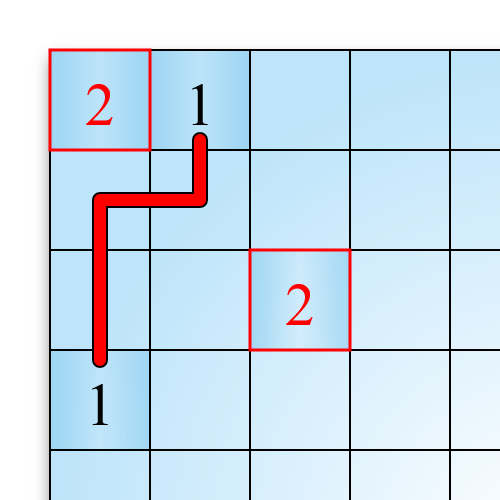
\includegraphics[width=0.3\textwidth]{images/falle_versuch.png}
        \caption{Die \glqq{Fallen}\grqq-Struktur und der Versuch des Lösungsprogramms}
        \label{abb:bild2}
    \end{center}
\end{figure}
